% !TeX encoding = UTF-8
% !TeX spellcheck = en_US


\documentclass[type=submission,name=IR]{oae}
% type = submission / final

% name = 
% JSS    default
% CS
% SW
% JCA
% IJS
% CES
% IR
% JMI

\usepackage{siunitx}
\usepackage{booktabs}
\usepackage{placeins}

\documentsetup{
  % No empty lines in the setup
  title = {A Protected Progressive Adaptive TTL Mechanism for Multi-Robot Task Allocation Under Limited Information Sharing},
  % Suggestions: No more than 16 words.
  % No abbreviations except for standardized ones.
  authors = {
    author1 = {
      name         = {Zi'an Fang},
      affiliations = {affil1},
    },
    author2 = {
      name         = {Yuchen Ye},
      affiliations = {affil1},
    },
    author3 = {
    	name         = {Wentao Zhang},
    	affiliations = {affil2},
    },
    author4 = {
    	name         = {Dandan Li},
    	affiliations = {affil1},
    },
  },
  affiliations = {
    affil1 = {
     School of Robotics and Intelligent Manufacturing, Huzhou Normal University, Huzhou 313000, Zhejiang, China.
    },
    affil2 = {
    School of Artificial Intelligence and Robotics, Hunan University, Changsha 410082, China	
    },
  },
  correspondence-to = {
Dandan Li
  },
  short-author      = {Fang \textit{et al}.},
  journal           = {Intelligence & Robotics},
  short-journal     = {Intell Robot},
  how-to-cite       = {},
  received          = {},
  first-decision    = {},
  revised           = {},
  accepted          = {},
  published         = {},
  academic-editor   = {},
  copy-editor       = {},
  production-editor = {},
  doi               = {},
  year              = {},
  volume            = {},
  end-page          = {},
}

% hyperref is always at the end of preamble
\usepackage{hyperref}



\begin{document}

\maketitle


\begin{abstract}
 Multi-robot systems are now being applied in an increasing number of fields. However, limited communication infrastructure in practical scenarios may require decentralized operation with local information sharing. Therefore, local communication mechanisms are critical for information sharing among robots. As the operational area expands, information sharing becomes increasingly difficult. Fixed TTL strategies do not adjust the propagation range to individual task needs, which may affect task allocation efficiency.
 To address this issue, this paper proposes a protected progressive adaptive time-to-live mechanism, namely PP-AT, for communication-efficient multi-robot task allocation under limited information sharing. When a task is released, the robot that first discovers the task becomes the source node. The source node calculates the TTL upper bound of the task using the collected task state and local robot state. Then, it propagates the task information from TTL = 1 and gradually expands the propagation range only when feasible candidate robots are insufficient. A protection mechanism uses state refresh and assignment awareness to maintain candidate information and guide subsequent propagation. Expansion stops when the candidate set satisfies the feasibility condition or when the TTL reaches the upper bound.
 The proposed method is evaluated in a NetFlood + MPDM environment and compared with fixed TTL baselines from 1 to 5. Simulation results show lower communication overhead than Fixed TTL = 2--5 in the tested settings, while Fixed TTL = 1 retains lower overhead.
 \paragraph{Keywords:} Multi-robot task allocation, limited information sharing, adaptive TTL, local communication, NetFlood, communication overhead
\end{abstract}





\section{1. Introduction}

In recent years, multi-robot systems have been widely applied in logistics, search and rescue, intelligent manufacturing, environmental monitoring, and other scenarios. Compared with traditional manual planning or single-robot systems, multi-robot systems have advantages in efficiency, robustness, and sustainability. Multi-robot task allocation (MRTA) is usually regarded as a core problem in multi-robot systems. It aims to reasonably assign tasks or goals to the most suitable robots according to indicators such as task urgency and required execution time.

Existing studies have examined communication constraints and localized information sharing in MRTA. Wang et al.~\cite{wang_eepi} studied the effects of communication topology, communication range, and perception range on distributed task allocation. Nayak et al.~\cite{nayak2025limited} used common TTL settings to examine the effects of limited information sharing on different allocation strategies. However, task requirements and local candidate availability can vary, so the same propagation range may not suit every task. This motivates task-specific control of message propagation according to task states and local robot information.

In localized information sharing, time-to-live (TTL) is a key factor because it determines the range of information sharing. Specifically, TTL is a mechanism that controls the number of hops for task-message propagation. However, a fixed TTL applies the same propagation range to all tasks, making it difficult to adapt to different task states, local robot distributions, and robot load conditions. When TTL is small, the communication overhead is low, but task visibility is limited, and the system may fail to find enough candidate robots. When TTL is large, task visibility is improved, but a large number of redundant messages may be generated, which reduces communication efficiency.

To address this issue, this paper proposes a protected progressive adaptive TTL method (PP-AT), which dynamically controls TTL according to task states and local robot states. The proposed method calculates a task-specific TTL upper bound based on four local state factors, and the communication range is progressively expanded only when the current range cannot provide sufficient feasible candidate robots. In this way, PP-AT avoids starting every task with a large TTL and allows expansion when one-hop information is insufficient.

During the progressive TTL expansion process, a protection mechanism is further introduced. This mechanism checks whether the current communication range can still support task allocation before deciding whether the task message should continue to be propagated. The purpose of this mechanism is to reduce repeated communication while avoiding degradation in the task completion rate caused by an overly small TTL.

The proposed mechanism is integrated into a NetFlood-based localized information sharing framework and evaluated with an MPDM-based task allocation method. Fixed TTL values from 1 to 5 are used as baseline methods. The evaluation metrics include the number of transmitted messages (MSG), the number of completed tasks (NTC), the message cost per completed task (MSG/NTC), total travel delay (TTD), and make-span time (MST). Experimental results show lower communication overhead relative to Fixed TTL = 2--5 with comparable mean task completion in the tested settings. Fixed TTL = 1 retains lower communication overhead.

The main contributions of this paper are summarized as follows:

\begin{itemize}
	\item A state-aware TTL upper bound estimation mechanism is proposed to adapt the communication range to task urgency, resource demand, candidate availability, and local load distribution.
	\item A protected progressive expansion mechanism is designed to reduce unnecessary message propagation while considering task allocation feasibility.
	\item The proposed PP-AT mechanism is integrated with task allocation algorithms under a limited information sharing framework and evaluated against Fixed TTL = 1--5.
	\item Experimental results show that PP-AT can reduce communication messages while maintaining comparable task completion performance, providing a practical trade-off between communication cost and allocation reliability.
\end{itemize}

The remainder of this paper is organized as follows. Section 2 presents the related work and problem formulation. Section 3 introduces the proposed PP-AT method. Section 4 describes the experimental settings and result analysis. Section 5 discusses the advantages and limitations of the proposed method, as well as the special case of Fixed TTL = 1. Section 6 concludes this paper.



\section{2. Related Work and Problem Formulation}

This section reviews existing studies related to multi-robot task allocation and limited information sharing. Then, the problem studied in this paper is formulated under a localized communication framework. The purpose of this section is to clarify the research context and define the communication-control problem addressed by the proposed PP-AT mechanism.

\subsection{2.1. Multi-Robot Task Allocation}

Existing MRTA methods aim to optimize various performance objectives, including task completion, travel distance, makespan or service time, energy consumption, and workload balance. Representative approaches include centralized optimization, distributed auction-based methods, heuristic and metaheuristic methods, and learning-based methods. These approaches differ not only in their optimization objectives and solution methods but also in the task structures and constraints they consider.

For multi-objective task allocation, Yu et al.~\cite{yu_mmoeadl} proposed a multimodal multi-objective optimization method combining deep reinforcement learning and large neighborhood search. Their method treats task allocation and path planning as a bi-level problem to provide multiple equivalent optimized solutions and improve computational efficiency. Martin et al.~\cite{martin_iterative_clustering} used iterative clustering to divide the global allocation problem into smaller subproblems and optimize robot--task assignments within each cluster, addressing tasks that require collaboration among heterogeneous robots. Dai et al.~\cite{dai_heterogeneous_rl} trained a decentralized task-selection policy through reinforcement learning. By considering robot capabilities and scheduling dependencies, their method reduces idle waiting during cooperation and shortens the overall completion time. In addition, Zhang et al.~\cite{zhang_energy_efficient} addressed time-window and task-precedence constraints through task batching and a batch solver, reducing the number of robots required and the energy consumed during task execution.

Although these studies improve MRTA through optimization, collaborative organization, and scheduling, their performance should be interpreted in light of their respective information-access assumptions. The task and robot states available to an allocator depend on the information-sharing mechanism. Therefore, the effects of communication range and local information on task allocation warrant further investigation.

\subsection{2.2 Limited Information Sharing and TTL-Based Communication}
The communication mechanism determines what information robots can obtain during task allocation. It is important to distinguish decentralized decision-making from localized information sharing. Dai et al.~\cite{dai_heterogeneous_rl} proposed a reinforcement learning method for heterogeneous multi-robot task allocation and scheduling, in which each robot independently selects its subsequent tasks. However, its execution still relies on global communication to collect broadcast information about task selections and robot working states. Therefore, discussions of decentralized task allocation methods should also clarify their information-sharing scope and communication assumptions.

For distributed task allocation, Wang et al.~\cite{wang_eepi} proposed an effective and efficient performance impact (EEPI) algorithm. By improving the cost function and task release procedure, the method increases the number of task allocations that satisfy task deadlines and robot fuel constraints. The study compared algorithm performance under different communication topologies, communication ranges, and perception ranges. It also noted that an insufficient communication range may prevent some robots from exchanging allocation information directly or indirectly, potentially leading to duplicate assignments. These findings indicate that information-access and exchange conditions affect both task visibility and allocation consistency among robots. The main improvements concern task allocation and convergence, rather than dynamically controlling message propagation hops for individual tasks.

Nayak et al.~\cite{nayak2025limited} further investigated the effects of limited information sharing on multi-robot task allocation. In their framework, task information, robot states, and allocation results are disseminated through NetFlood, with a common TTL setting used to limit the propagation range. The study compared MPDM, RBTS, and MARL with their localized versions and varied TTL to examine the relationship between communication message counts and task allocation performance. Using common TTL settings to compare different propagation ranges, the results showed that a larger TTL increases message transmission but does not necessarily provide corresponding gains in task completion in the tested scenarios.

Building on these studies, this paper focuses on controlling task-message propagation according to allocation needs. Instead of applying a common TTL setting to all tasks, PP-AT estimates a propagation upper bound from the task state and the source robot's local information. Propagation starts from one hop and expands progressively, with candidate states and allocation results informing subsequent propagation decisions. The mechanism does not replace the existing task allocator. Instead, it adjusts message propagation within a localized information-sharing framework to reduce unnecessary communication and evaluate the effects on task completion performance.
\subsection{2.3 Problem Formulation}

The problem considered in this paper is based on a decentralized multi-robot task allocation system in a two-dimensional workspace. The robot set is denoted as $\mathcal{R}=\{r_1,r_2,\ldots,r_m\}$, and the task set is denoted as $\mathcal{T}=\{\tau_1,\tau_2,\ldots,\tau_n\}$. Tasks are dynamically released during the mission process, and task allocation decisions are made based on locally available information. For each robot $r_i$, its state at time $t$ is defined as
\[
r_i(t)=\left(p_i(t),q_i(t),s_i(t),l_i(t)\right),
\]
where $p_i(t)$ denotes the position of robot $r_i$, $q_i(t)$ denotes its remaining resource, $s_i(t)\in\{\mathrm{idle},\mathrm{busy}\}$ denotes its working state, and $l_i(t)$ denotes its current load. For each task $\tau_j$, its state is defined as
\[
\tau_j=\left(p_j,a_j,\rho_j,q_j,E_j\right),
\]
where $p_j$ denotes the task position, $a_j$ denotes the release time, $\rho_j$ denotes the task priority, $q_j$ denotes the required resource, and $E_j$ denotes the execution time. A task is regarded as completed when the assigned robot reaches the task location, finishes the execution period, and consumes the required resource.

The communication relationship among robots is modeled as a dynamic graph
\[
G(t)=\left(\mathcal{R},\mathcal{E}(t)\right).
\]
An edge exists between two robots if their Euclidean distance is not larger than the communication radius $d_c$:
\[
(r_i,r_k)\in\mathcal{E}(t), \quad \mathrm{if}\ \|p_i(t)-p_k(t)\|\leq d_c.
\]
After a task $\tau_j$ is released at $a_j$, the robot that first discovers it at $t_j\geq a_j$ becomes the source node, denoted as $s_j$. The task message is then propagated through the communication graph by NetFlood. The propagation range is controlled by the time-to-live value $h_j$, where $h_j\in\{1,2,3,4,5\}$. At a decision time $t$, an idealized feasible candidate set based on the current communication graph and actual robot states is
\[
\mathcal{C}^{\mathrm{ideal}}_j(h_j,t)=
\left\{
r_i\in\mathcal{R}
\,\middle|\,
H_{s_j i}(t)\leq h_j,\ 
s_i(t)=\mathrm{idle},\
q_i(t)\geq q_j
\right\}.
\]
where $H_{s_j i}(t)$ denotes the shortest hop distance in $G(t)$. This idealized set describes the basic communication, state, and resource requirements; the source node does not directly observe all actual robot states. During progressive propagation, movement and report delays can make the received information differ from this instantaneous set. PP-AT therefore uses the reported-state sets defined in Section~3.3 for its decisions, including an estimated completion-time check. The selected robot checks its own availability and resource before accepting an assignment. The key notations and their descriptions used hereafter are listed in Table~\ref{tab:1}.

\begin{table}[htb]
	\centering
	\caption{Notation Descriptions}
	\label{tab:1}
	\begin{tabular}{lp{0.68\linewidth}}
		\toprule
		Notation & Description \\
		\midrule
		$\mathcal{R}=\{r_1,r_2,\ldots,r_m\}$ & Set of robots \\
		$\mathcal{T}=\{\tau_1,\tau_2,\ldots,\tau_n\}$ & Set of tasks \\
		$r_i$ & The $i$th robot \\
		$\tau_j$ & The $j$th task \\
		$p_i(t)$ & Position of robot $r_i$ at time $t$ \\
		$q_i(t)$ & Remaining resource of robot $r_i$ \\
		$s_i(t)$ & Working state of robot $r_i$ \\
		$l_i(t)$ & Current load of robot $r_i$ \\
		$p_j$ & Position of task $\tau_j$ \\
		$a_j$ & Release time of task $\tau_j$ \\
		$\rho_j$ & Priority of task $\tau_j$ \\
		$q_j$ & Required resource of task $\tau_j$ \\
		$E_j$ & Execution time of task $\tau_j$ \\
		$t$ & Current decision time \\
		$H_j$ & TTL upper bound of task $\tau_j$ \\
		$h_j$ & Current propagation TTL of task $\tau_j$ \\
		$G(t)$ & Dynamic communication graph among robots \\
		$\mathcal{E}(t)$ & Set of communication edges at time $t$ \\
		$d_c$ & Communication radius of each robot \\
		$s_j$ & Source robot that first discovers task $\tau_j$ \\
		$t_j$ & Discovery time of task $\tau_j$ \\
		$H_{s_j i}(t)$ & Shortest communication hop distance from $s_j$ to $r_i$ at time $t$ \\
		$\mathcal{C}^{\mathrm{ideal}}_j(h_j,t)$ & Idealized feasible candidate set at time $t$ \\
		$N_{\mathrm{TC}}$ & Number of completed tasks \\
		$M_{\mathrm{SG}}$ & Number of transmitted messages \\
		$M_{\mathrm{SG}}/N_{\mathrm{TC}}$ & Messages per completed task \\
		\bottomrule
	\end{tabular}
\end{table}

To ensure a fair comparison with the localized information sharing framework in the reference study, the main evaluation metrics follow the baseline study~\cite{nayak2025limited}, including NTC, MSG, TTD, and MST. Their aggregation rules in this implementation are specified in Section~4.1. In addition, MSG/NTC is further introduced as a derived metric to evaluate the communication cost required for each completed task. It should be noted that the proposed PP-AT algorithm is not a new task allocator designed to replace allocators such as MPDM. Instead, PP-AT acts as a communication-control mechanism that adjusts the propagation range of task messages before the task allocator takes effect. In summary, the problem studied in this paper is to determine a task-specific TTL for each dynamically released task under localized information sharing, so that communication overhead can be reduced while maintaining the number of completed tasks.



\section{3. Proposed Method}

\subsection{3.1 Overview of PP-AT}
This section introduces the protected progressive adaptive TTL method, namely PP-AT. PP-AT is not designed as a new task allocator. Instead, it determines the propagation range of task messages, i.e., the TTL, before the task allocator takes effect, aiming to reduce communication overhead while maintaining the number of completed tasks.

\subsection{3.2 State-Aware TTL Upper Bound Estimation}
For each dynamically released task, PP-AT first estimates the required TTL upper bound according to the task state observed by the source robot and the robot states within the one-hop communication range of the source robot. This TTL upper bound determines the maximum propagation range allowed during message expansion. The purpose of this design is to avoid propagating every task message throughout the entire local network, while still allowing the propagation range to be enlarged when the candidate robots within the current TTL are insufficient.
For task $\tau_j$, the one-hop neighborhood of the source robot $s_j$ is defined as
\[
\mathcal{N}_1(s_j)=
\left\{
r_i\in\mathcal{R}
\mid
\|p_i(t_j)-p_{s_j}(t_j)\|\leq d_c
\right\}.
\]
Based on the one-hop neighborhood information obtained from $\mathcal{N}_1(s_j)$, four state factors, namely $P_j$, $R_j$, $C_j$, and $L_j$, are selected to calculate the TTL upper bound. These four factors describe the task urgency, resource demand, candidate sufficiency, and local load imbalance, respectively. A higher $P_j$ or $R_j$ indicates that the task may require a larger propagation range, while a higher $C_j$ means that sufficient feasible robots can already be found in the one-hop neighborhood. In addition, a higher $L_j$ indicates a more imbalanced local workload, which may require a larger search range to improve allocation reliability. The detailed definitions of these factors are listed in Table~\ref{tab:2}.

\begin{table}[htb]
	\centering
	\caption{State Factors Used in TTL Upper Bound Estimation}
	\label{tab:2}
	\begin{tabular}{lp{0.52\linewidth}p{0.18\linewidth}}
		\toprule
		Symbol & Description & Range \\
		\midrule
		$P_j$ & Normalized priority of task $\tau_j$ & $[0,1]$ \\
		$R_j$ & Normalized resource demand of task $\tau_j$ & $[0,1]$ \\
		$C_j$ & Candidate robot sufficiency in $\mathcal{N}_1(s_j)$ & $[0,1]$ \\
		$L_j$ & Local load imbalance in $\mathcal{N}_1(s_j)$ & $[0,1]$ \\
		$N_{\mathrm{candidate}}$ & Number of feasible candidate robots in $\mathcal{N}_1(s_j)$ & $\mathbb{Z}_{\geq 0}$ \\
		$q_j$ & Required resource of task $\tau_j$ & $[r_{\min},r_{\max}]$ \\
		$r_{\min}$ & Minimum task resource demand & positive scalar \\
		$r_{\max}$ & Maximum task resource demand & positive scalar \\
		$N_{\mathrm{ref}}$ & Reference number of sufficient candidate robots & positive scalar \\
		$\epsilon$ & Small constant used to avoid division by zero & positive scalar \\
		$\theta_0$ & Basic propagation demand coefficient & scalar \\
		$\theta_1$ & Weight of task priority & scalar \\
		$\theta_2$ & Weight of task resource demand & scalar \\
		$\theta_3$ & Weight of candidate sufficiency & scalar \\
		$\theta_4$ & Weight of local load imbalance & scalar \\
		$\mathrm{load}$ & Load vector of robots in $\mathcal{N}_1(s_j)$ & vector \\
		$\operatorname{std}(\mathrm{load})$ & Standard deviation of local robot loads & non-negative scalar \\
		$\operatorname{mean}(\mathrm{load})$ & Mean value of local robot loads & non-negative scalar \\
		\bottomrule
	\end{tabular}
\end{table}
The four state factors are normalized to $[0,1]$ as follows.
\[
P_j=\operatorname{clip}_{[0,1]}(\rho_j),
\]

\[
R_j=\operatorname{clip}_{[0,1]}\left(\frac{q_j-r_{\min}}{r_{\max}-r_{\min}}\right),
\]

\[
C_j=\operatorname{clip}_{[0,1]}
\left(
\frac{N_{\mathrm{candidate}}}{N_{\mathrm{ref}}}
\right),
\]

\[
L_j=\operatorname{clip}_{[0,1]}
\left(
\frac{\operatorname{std}(\mathrm{load})}
{\operatorname{mean}(\mathrm{load})+\epsilon}
\right).
\]
The reference count $N_{\mathrm{ref}}$ normalizes candidate sufficiency; it does not set the expansion stopping threshold. A small constant $\epsilon>0$ prevents division by zero. Clipping is defined by
\begin{equation}
\operatorname{clip}_{[a,b]}(x)=\min\{b,\max\{a,x\}\},\qquad a\leq b.
\label{eq:clip_definition}
\end{equation}
These factors determine the task-specific TTL upper bound through a weighted score:
\[
H_j=
\operatorname{clip}_{[1,5]}
\left(
\operatorname{round}
\left(
\theta_0+\theta_1P_j+\theta_2R_j-\theta_3C_j+\theta_4L_j
\right)
\right).
\]
The coefficient $\theta_0$ sets the base score, and $\theta_1$--$\theta_4$ weight priority, resource demand, candidate sufficiency, and load imbalance, respectively. Parameter values are reported in the experimental settings.
\subsection{3.3 Protected Progressive Expansion}
PP-AT starts propagation at $h_j=1$ and uses $H_j$ as the expansion limit. After each round, the source node checks candidate feasibility from received robot-state reports and decides whether to allocate, wait, or expand.

Let $\mathcal{V}_j(h_j,t)$ contain the robots regarded as visible under TTL $h_j$ with valid state reports at the source. For robot $r_i$, these reports give its position $\widehat p_i$, remaining resource $\widehat q_i$, and busy-until time $\widehat B_i$. Its estimated task completion time is
\begin{equation}
\widehat T_{ij}(t)=\max\{\widehat B_i,t\}
+\frac{\|\widehat p_i-p_j\|}{v}+E_j,
\label{eq:estimated_completion}
\end{equation}
Here, $v$ is the robot speed and $E_j$ is the execution time. Because reports may become outdated, this estimate does not guarantee completion. Robots with sufficient resources and estimated completion by the simulation end time $T_{\mathrm{end}}$ form
\begin{equation}
\mathcal{F}_j(h_j,t)=\left\{r_i\in\mathcal{V}_j(h_j,t)\mid
\widehat q_i\geq q_j,\ \widehat T_{ij}(t)\leq T_{\mathrm{end}}\right\},
\label{eq:completable_candidates}
\end{equation}
Among these robots, those reported as idle form the immediately feasible candidate set:
\begin{equation}
\mathcal{C}^{\mathrm{imm}}_j(h_j,t)=
\left\{r_i\in\mathcal{F}_j(h_j,t)\mid\widehat B_i\leq t\right\}.
\label{eq:immediate_candidates}
\end{equation}
Propagation stops and task allocation begins once
\begin{equation}
\left|\mathcal{C}^{\mathrm{imm}}_j(h_j,t)\right|\geq1.
\label{eq:progressive_ready}
\end{equation}

Otherwise, PP-AT considers waiting before expanding. Task priority determines the waiting threshold:
\begin{equation}
W_j=W_{\max}-(W_{\max}-W_{\min})P_j,
\label{eq:waiting_threshold}
\end{equation}
The bounds $W_{\min}$ and $W_{\max}$ specify the allowed threshold range. The shortest reported wait within $\mathcal{F}_j(h_j,t)$ is
\begin{equation}
w_j(t)=\begin{cases}
\displaystyle\min_{r_i\in\mathcal{F}_j(h_j,t)}\max\{\widehat B_i-t,0\},
&\mathcal{F}_j(h_j,t)\neq\varnothing,\\
+\infty,&\mathcal{F}_j(h_j,t)=\varnothing.
\end{cases}
\label{eq:local_wait}
\end{equation}
For $w_j(t)\leq W_j$, PP-AT retains the current TTL and rechecks at $t+\max\{\Delta_c,w_j(t)\}$, with $\Delta_c$ denoting the collection interval. Setting $W_{\min}=10$~s and $W_{\max}=60$~s gives $W_j=60-50P_j$ seconds.

When $\mathcal{C}^{\mathrm{imm}}_j(h_j,t)=\varnothing$, $w_j(t)>W_j$, and $h_j<H_j$, propagation expands by one hop:
\begin{equation}
h_j\leftarrow h_j+1.
\label{eq:ttl_expansion}
\end{equation}
A further $2\Delta_c$ interval allows message propagation and state collection before reassessment. At $h_j=H_j$, waiting remains possible when $w_j(t)\leq W_j$; otherwise, the controller terminates without implying successful allocation or completion. These rules limit unnecessary propagation while allowing a wider search when local candidates cannot serve the task promptly.

The protection mechanism also maintains the state reports used in these decisions. Let $\widehat t_i$ be the timestamp of a stored report. A visible remote robot with reported resource $\widehat q_i\geq q_j$ refreshes its state when
\begin{equation}
t-\widehat t_i\geq A_{\max}.
\label{eq:report_age}
\end{equation}
The refresh uses NetFlood with the current TTL and is included in StateMSG. The report is updated only if it reaches the source; otherwise, the robot is removed from the current visible and reported sets. The source updates its own state locally. In addition, sources reached by an existing allocation-result dissemination update the reported busy-until time and load of the assigned robot for other pending tasks that already contain its report. Their decisions are then scheduled for reassessment after $\Delta_c$. This reuses the counted allocation dissemination rather than assuming a system-wide state update.

To reduce repeated forwarding during expansion, each task retains its reached-node set and forwarding history. Only nodes on the current propagation frontier that have not forwarded this task message send it to their current neighbors. A node forwards at most once during the task flood, while each outgoing neighbor copy is counted, including copies received by nodes that already know the task. State reports are cached between expansion rounds, with stale reports refreshed as described above. Consequently, the reached set depends on the propagation history and need not equal the instantaneous hop neighborhood in $G(t)$.

\subsection{3.4 Integration with MPDM}
To reproduce the conclusions of the reference study as closely as possible, this paper adopts the MPDM + NetFlood framework and integrates the proposed PP-AT mechanism into it. PP-AT is used to determine the propagation range of task messages, while the MPDM allocator is used to complete task allocation among candidate robots that receive the task messages.

For each dynamically released task, the source robot first calculates the TTL upper bound of the task, and the protected progressive expansion mechanism is then applied to determine the final propagation range. After that, MPDM performs task allocation based on the candidate robot set formed within the determined propagation range.

It should be stated that PP-AT controls task-message propagation, waiting, and reported-state updates, and does not change the task allocation rules of MPDM. Therefore, when compared with fixed-TTL methods, the differences in the obtained results mainly come from the change in the communication-control mechanism.




\section{4. Experiments and Results}
This section evaluates the effectiveness of the proposed PP-AT method through simulation experiments. The experiments are conducted based on the NetFlood + MPDM framework, and the PP-AT method is compared with fixed-TTL baseline methods from Fixed TTL = 1 to Fixed TTL = 5. The evaluation focuses on whether PP-AT can reduce communication overhead while maintaining task completion performance.
\subsection{4.1 Experimental Setup}
The experiments are conducted in a two-dimensional decentralized multi-robot task allocation environment. After tasks are dynamically released, task messages are propagated through the NetFlood protocol, and task allocation is completed by the MPDM allocator. To verify the effectiveness of the proposed PP-AT mechanism, it is compared with five fixed-TTL baseline methods, namely Fixed TTL = 1, Fixed TTL = 2, Fixed TTL = 3, Fixed TTL = 4, and Fixed TTL = 5.

To ensure a fair comparison, all methods are evaluated under the same task scenarios, robot settings, and random seeds. In the experiments, the TTL upper bound uses the fixed heuristic coefficients reported in Table~\ref{tab:exp_parameters}, together with normalized task resource demand and candidate sufficiency. The evaluation metrics include the number of completed tasks (NTC), the number of transmitted messages (MSG), messages per completed task (MSG/NTC), total travel delay (TTD), and make-span time (MST). The main experimental parameters are listed in Table~\ref{tab:exp_parameters}.
\begin{table}[htb]
	\centering
	\caption{Experimental Parameters}
	\label{tab:exp_parameters}
	\begin{tabular}{ll}
		\toprule
		Parameter & Value \\
		\midrule
		Workspace size & $1000 \times 1000$ m \\
		Number of robots & 60 \\
		Maximum number of tasks & 1000 \\
		Simulation time & 500 s \\
		Time step & 1 s \\
		Task arrival rate & 2 tasks/s (exponential interarrival times) \\
		Task release mode & Dynamic release \\
		Task centers & $(250,250)$, $(700,250)$, $(250,700)$, $(700,700)$ \\
		Task cluster standard deviation & 150 m \\
		Communication protocol & NetFlood \\
		Task allocator & MPDM; lightweight MARL (auxiliary) \\
		Communication radius & 100 m \\
		Task discovery radius & 50 m \\
		Robot speed & 10 m/s \\
		Initial robot resource & 70 \\
		Task resource demand & $[8,25]$ \\
		Task execution time & $[10,30]$ s \\
		TTL range & $[1,5]$ \\
		Compared methods & Fixed TTL = 1--5, PP-AT \\
		Number of random seeds & 20 per allocator group \\
		MPDM random seeds & 75001--75020 \\
		MARL random seeds & 77001--77020 \\
		Collection interval $\Delta_c$ & 1 s \\
		Waiting thresholds $(W_{\min},W_{\max})$ & (10, 60) s \\
		State refresh threshold $A_{\max}$ & 5 s \\
		$\theta_0$ & 1.7 \\
		$\theta_1$ & 0.5 \\
		$\theta_2$ & 0.4 \\
		$\theta_3$ & 1.2 \\
		$\theta_4$ & 0.3 \\
		$N_{\mathrm{ref}}$ & 2 \\
		$\epsilon$ & $10^{-6}$ \\
		Message counting mode & Link copies \\
		\bottomrule
	\end{tabular}
\end{table}

The environment follows the workspace geometry, task clusters, robot speed, discovery radius, and execution-time range stated in the reference study~\cite{nayak2025limited}. The 60-robot, 2-tasks/s case is used as the base setting. Parameters not fully specified in that study are explicit implementation assumptions: a 500-s horizon, a 1-s time step and collection interval, exponential task interarrival times, uniform resource demand in $[8,25]$, uniform priority in $[0,1]$, and deterministic random-waypoint exploration by idle robots. Initial robot positions are sampled uniformly over the workspace. Task locations are sampled around the four centers with equal probability and clipped to the workspace boundary; resource demand and execution time are continuous uniform samples. This is a reference-aligned reconstruction, rather than an exact reproduction of the original simulator. Communication is limited by range, topology, and TTL; the model does not simulate a bandwidth cap, packet loss, MAC contention, or delay jitter.

An auxiliary comparison uses a lightweight shared-policy MARL allocator implemented for this study, rather than an exact reproduction of the reference MARL network. Its actor and critic each have hidden layers of 64 and 32 units. A 65-dimensional observation supports up to ten task choices and a no-operation action. Robots propose tasks from masked action probabilities; conflicts are resolved by proposal probability, with robot index breaking ties. Training uses 210 episodes of 120 s with mixed visibility settings (Global, Fixed TTL = 1--5, and Adaptive TTL). The saved checkpoint is shared by all six MARL test methods. Test actions are deterministic, with no training or exploration. MPDM uses seeds 75001--75020 and MARL uses 77001--77020; pairing applies within each group, not between the two allocators. Reported table entries are the mean and sample standard deviation over the 20 seeds.

Following the terminology in the reference study, TTD is the accumulated travel time and MST is the sum of travel and execution times, both measured in seconds. Let $\mathcal{A}_{\mathrm{acc}}$ contain the robot--task assignments accepted during the simulation, and let $d_{ij}^{\mathrm{assign}}$ be the travel distance at acceptance. The implemented aggregates are
\begin{equation}
\mathrm{TTD}=\sum_{(i,j)\in\mathcal{A}_{\mathrm{acc}}}
\frac{d_{ij}^{\mathrm{assign}}}{v},\qquad
\mathrm{MST}=\sum_{(i,j)\in\mathcal{A}_{\mathrm{acc}}}
\left(\frac{d_{ij}^{\mathrm{assign}}}{v}+E_j\right).
\label{eq:time_metrics}
\end{equation}
Both totals are recorded when an assignment is accepted, including planned travel and execution for accepted tasks unfinished at the horizon. This aggregation convention is stated explicitly because the reference description does not resolve that boundary case. MST here follows the reference's additive definition rather than the maximum completion time across robots. NTC counts only tasks completed by the horizon. For each seed, MSG/NTC is computed from that run's totals, and the table reports the mean of these per-run ratios.

Communication overhead includes all three protocol phases:
\begin{equation}
\mathrm{MSG}=\mathrm{TaskMSG}+\mathrm{StateMSG}+\mathrm{AllocationMSG}.
\label{eq:message_metrics}
\end{equation}
TaskMSG counts task announcements and progressive forwarding. StateMSG counts robot-state replies, refreshes, and any retry-related state communication performed by the simulator. AllocationMSG counts allocation-result dissemination with twice the task's current TTL. All phases use the same link-copy rule: one outgoing copy to one adjacent robot counts as one message, so a transmission to $k$ neighbors counts as $k$ messages. This is a count of transmitted copies, not unique payloads or over-the-air broadcast events. The fixed-TTL baselines retain a fixed task-message range; PP-AT additionally uses incremental forwarding and report maintenance, whose messages are included in the same totals.

\subsection{4.2 Comparison With Fixed-TTL Baselines}

This section first evaluates PP-AT under the MPDM allocator, which is the main experimental setting of this paper. To further check whether the proposed communication-control mechanism depends on a specific allocator, an auxiliary MARL-based comparison is also reported. In both groups, PP-AT is compared with Fixed TTL = 1 to Fixed TTL = 5 under the same NetFlood-based information sharing framework.

Table~\ref{tab:main_results} summarizes the main comparison results between PP-AT + MPDM and the fixed-TTL baselines, while Table~\ref{tab:marl_results} reports the corresponding auxiliary results under MARL. Within each allocator group, all methods are evaluated with the same task scenarios, robot settings, and paired random seeds.

\begin{table}[htb]
\centering
\caption{Main Comparison Results Under MPDM}
\label{tab:main_results}
\begin{tabular}{lccccc}
\toprule
Method & NTC & MSG & MSG/NTC & TTD (s) & MST (s) \\
\midrule
Fixed TTL = 1 & $255.50 \pm 4.27$ & $9634.60 \pm 866.84$ & $37.70 \pm 3.28$ & $1335.10 \pm 69.94$ & $6425.04 \pm 137.68$ \\
Fixed TTL = 2 & $254.45 \pm 4.08$ & $52462.15 \pm 8190.95$ & $206.41 \pm 33.82$ & $1587.00 \pm 47.70$ & $6642.61 \pm 119.98$ \\
Fixed TTL = 3 & $255.10 \pm 3.80$ & $108466.40 \pm 16423.20$ & $425.72 \pm 67.99$ & $1784.20 \pm 98.50$ & $6871.55 \pm 154.18$ \\
Fixed TTL = 4 & $255.00 \pm 3.60$ & $175177.70 \pm 37142.83$ & $687.75 \pm 148.95$ & $1875.50 \pm 103.41$ & $6954.40 \pm 163.34$ \\
Fixed TTL = 5 & $255.05 \pm 3.82$ & $243248.90 \pm 49507.70$ & $954.77 \pm 199.70$ & $1958.91 \pm 126.51$ & $7039.07 \pm 182.17$ \\
PP-AT & $255.50 \pm 4.29$ & $16269.50 \pm 1956.21$ & $63.72 \pm 7.92$ & $1383.62 \pm 57.81$ & $6476.55 \pm 160.62$ \\
\bottomrule
\end{tabular}
\end{table}

As shown in Tables~\ref{tab:main_results} and~\ref{tab:marl_results}, PP-AT achieves a similar mean NTC to the fixed-TTL baselines under both MPDM and MARL. These mean values alone do not establish statistical equivalence. The corresponding MSG and MSG/NTC comparisons are presented in Figs.~\ref{fig:msg_comparison} and~\ref{fig:msg_per_ntc_comparison} for MPDM, and in Figs.~\ref{fig:marl_msg_comparison} and~\ref{fig:marl_msg_per_ntc_comparison} for MARL. Tables report mean $\pm$ sample standard deviation across 20 paired seeds within each allocator group.

\begin{figure}[!htbp]
\centering
\begin{minipage}{0.48\linewidth}
\centering
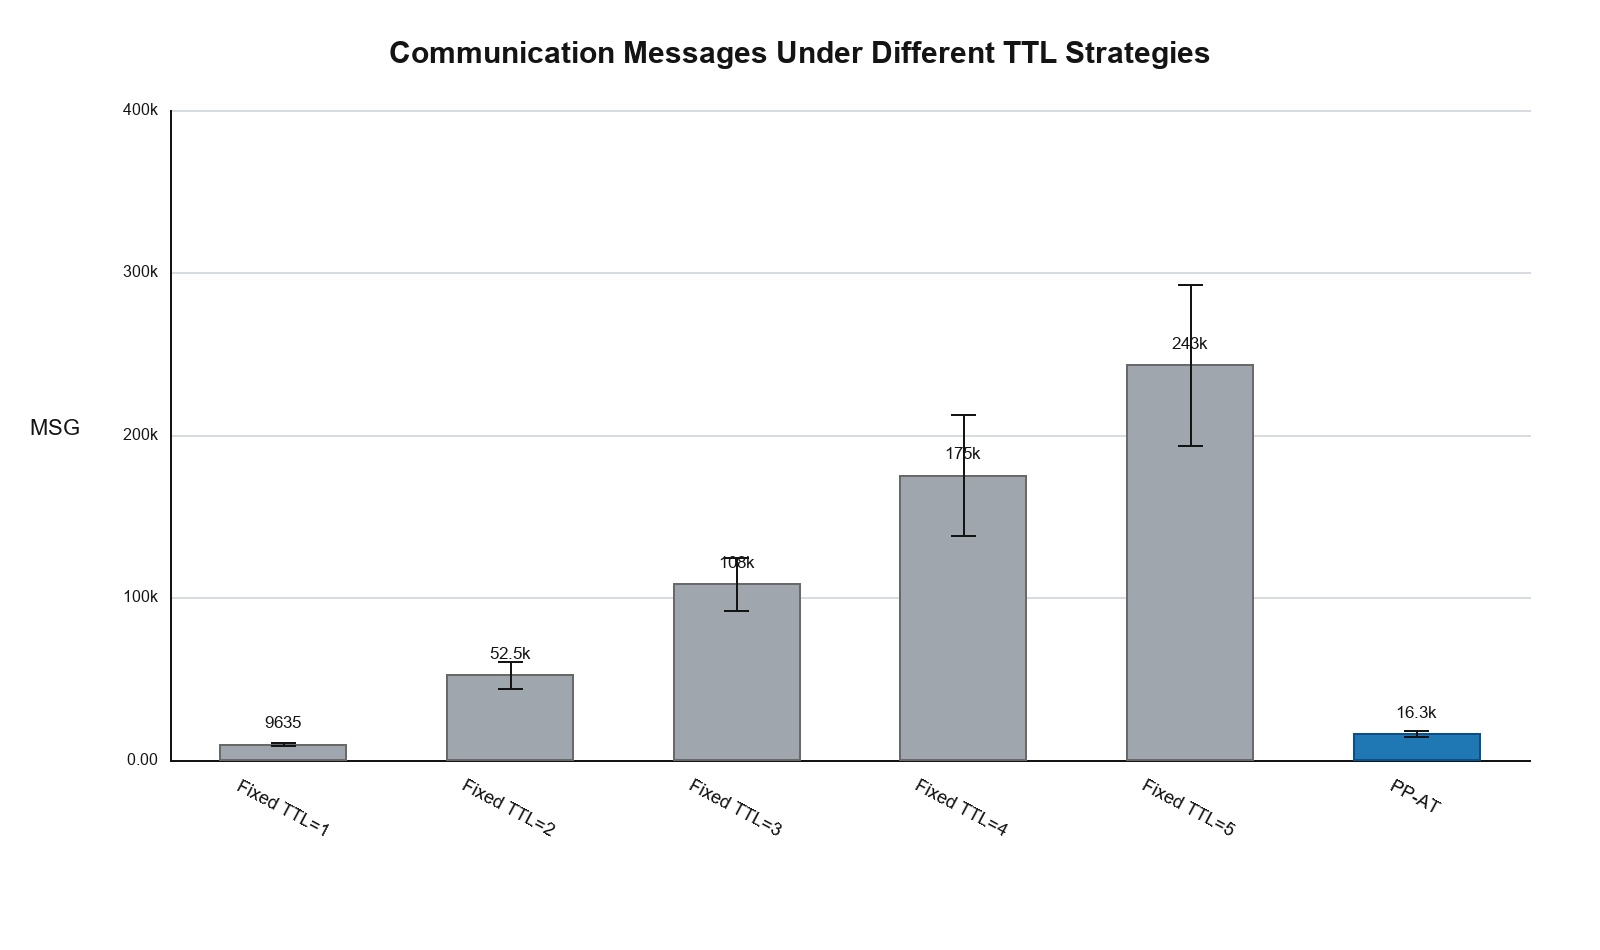
\includegraphics[width=\linewidth]{figures/fig1_msg_comparison.jpg}
\captionof{figure}{MSG comparison under MPDM (mean $\pm$ sample standard deviation).}
\label{fig:msg_comparison}
\end{minipage}\hfill
\begin{minipage}{0.48\linewidth}
\centering
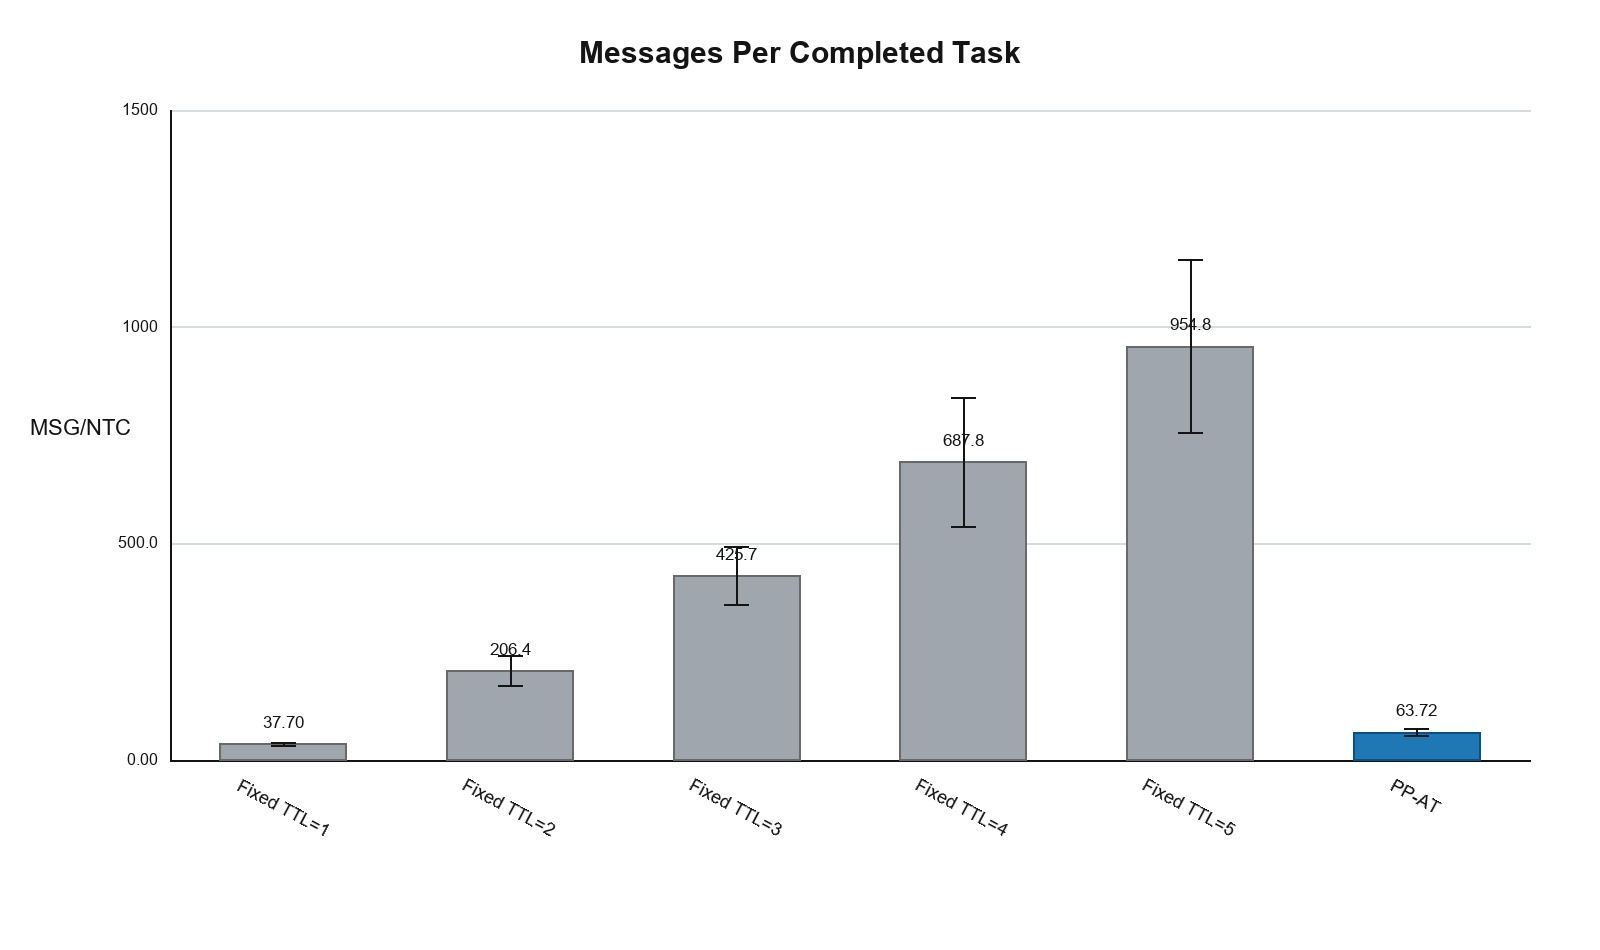
\includegraphics[width=\linewidth]{figures/fig3_msg_per_ntc_comparison.jpg}
\captionof{figure}{MSG/NTC comparison under MPDM (mean $\pm$ sample standard deviation).}
\label{fig:msg_per_ntc_comparison}
\end{minipage}
\end{figure}

The MSG results under MPDM and MARL, shown in Figs.~\ref{fig:msg_comparison} and~\ref{fig:marl_msg_comparison}, exhibit the same overall tendency: the number of transmitted messages increases rapidly when the fixed TTL is enlarged from 2 to 5. Compared with these larger fixed-TTL settings, PP-AT substantially reduces redundant message propagation under both allocators. However, Fixed TTL = 1 still has the lowest communication overhead because it always uses the minimum propagation range.

To account for differences in completed task counts, MSG/NTC is compared in Figs.~\ref{fig:msg_per_ntc_comparison} and~\ref{fig:marl_msg_per_ntc_comparison}. Under both MPDM and MARL, PP-AT achieves a lower mean MSG/NTC than Fixed TTL = 2 to Fixed TTL = 5. Thus, the communication savings remain when measured per completed task. This result does not imply that task completion is unchanged in every run.

\begin{figure}[!htbp]
\centering
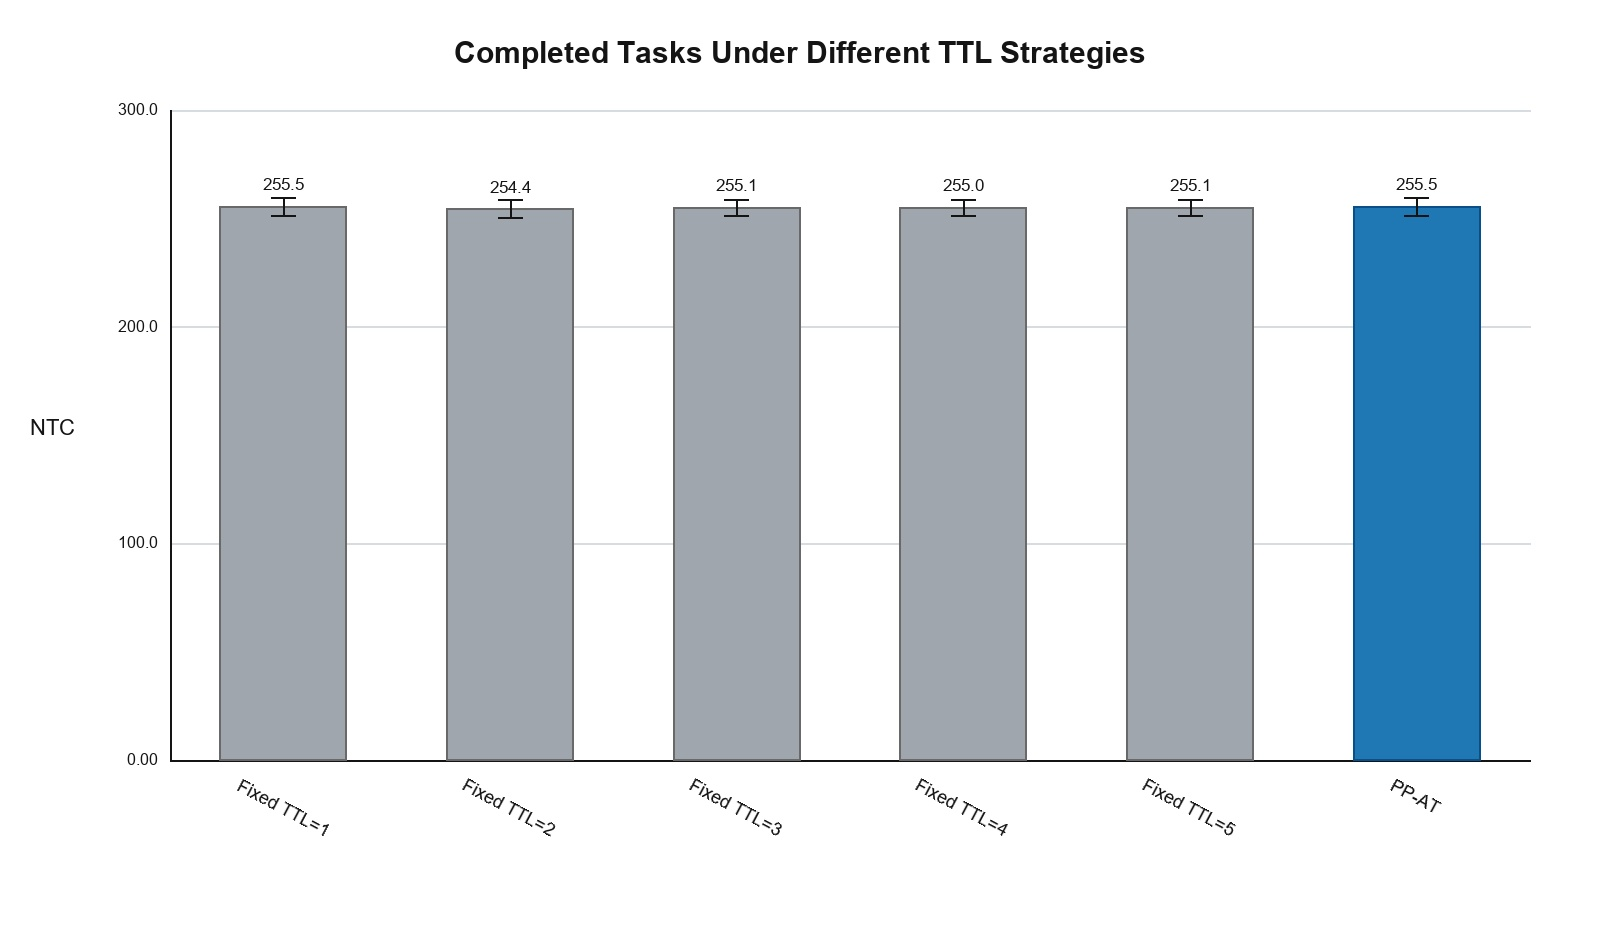
\includegraphics[width=0.46\linewidth]{figures/fig2_ntc_comparison.jpg}
\caption{NTC comparison under MPDM (mean $\pm$ sample standard deviation).}
\label{fig:ntc_comparison}
\end{figure}

The task completion results in Figs.~\ref{fig:ntc_comparison} and~\ref{fig:marl_ntc_comparison} show that mean NTC values remain close under both allocators in the tested setting. Together with the communication results, they indicate a favorable average trade-off relative to Fixed TTL = 2--5. The consistent trends provide auxiliary evidence for applying PP-AT with the two tested allocators, rather than establishing generalization to all allocation algorithms.




\begin{table}[htb]
\centering
\caption{Auxiliary Comparison Results Under MARL}
\label{tab:marl_results}
\begin{tabular}{lccccc}
\toprule
Method & NTC & MSG & MSG/NTC & TTD (s) & MST (s) \\
\midrule
Fixed TTL = 1 & $255.75 \pm 4.58$ & $7283.00 \pm 449.63$ & $28.48 \pm 1.78$ & $1548.22 \pm 65.38$ & $6707.50 \pm 182.96$ \\
Fixed TTL = 2 & $253.45 \pm 4.76$ & $45218.70 \pm 5193.23$ & $178.35 \pm 19.76$ & $2110.20 \pm 129.23$ & $7205.69 \pm 207.94$ \\
Fixed TTL = 3 & $254.70 \pm 5.35$ & $98358.25 \pm 16949.81$ & $386.59 \pm 68.28$ & $2542.21 \pm 157.38$ & $7676.22 \pm 217.73$ \\
Fixed TTL = 4 & $253.75 \pm 4.96$ & $169334.00 \pm 36773.96$ & $666.73 \pm 139.85$ & $2867.40 \pm 199.43$ & $7974.29 \pm 287.87$ \\
Fixed TTL = 5 & $253.80 \pm 5.34$ & $269748.65 \pm 59998.66$ & $1062.55 \pm 233.85$ & $3142.89 \pm 214.00$ & $8234.56 \pm 307.97$ \\
PP-AT & $254.90 \pm 4.76$ & $13098.45 \pm 853.83$ & $51.40 \pm 3.51$ & $1588.91 \pm 65.10$ & $6719.01 \pm 190.04$ \\
\bottomrule
\end{tabular}
\end{table}



\begin{figure}[!htbp]
\centering
\begin{minipage}{0.48\linewidth}
\centering
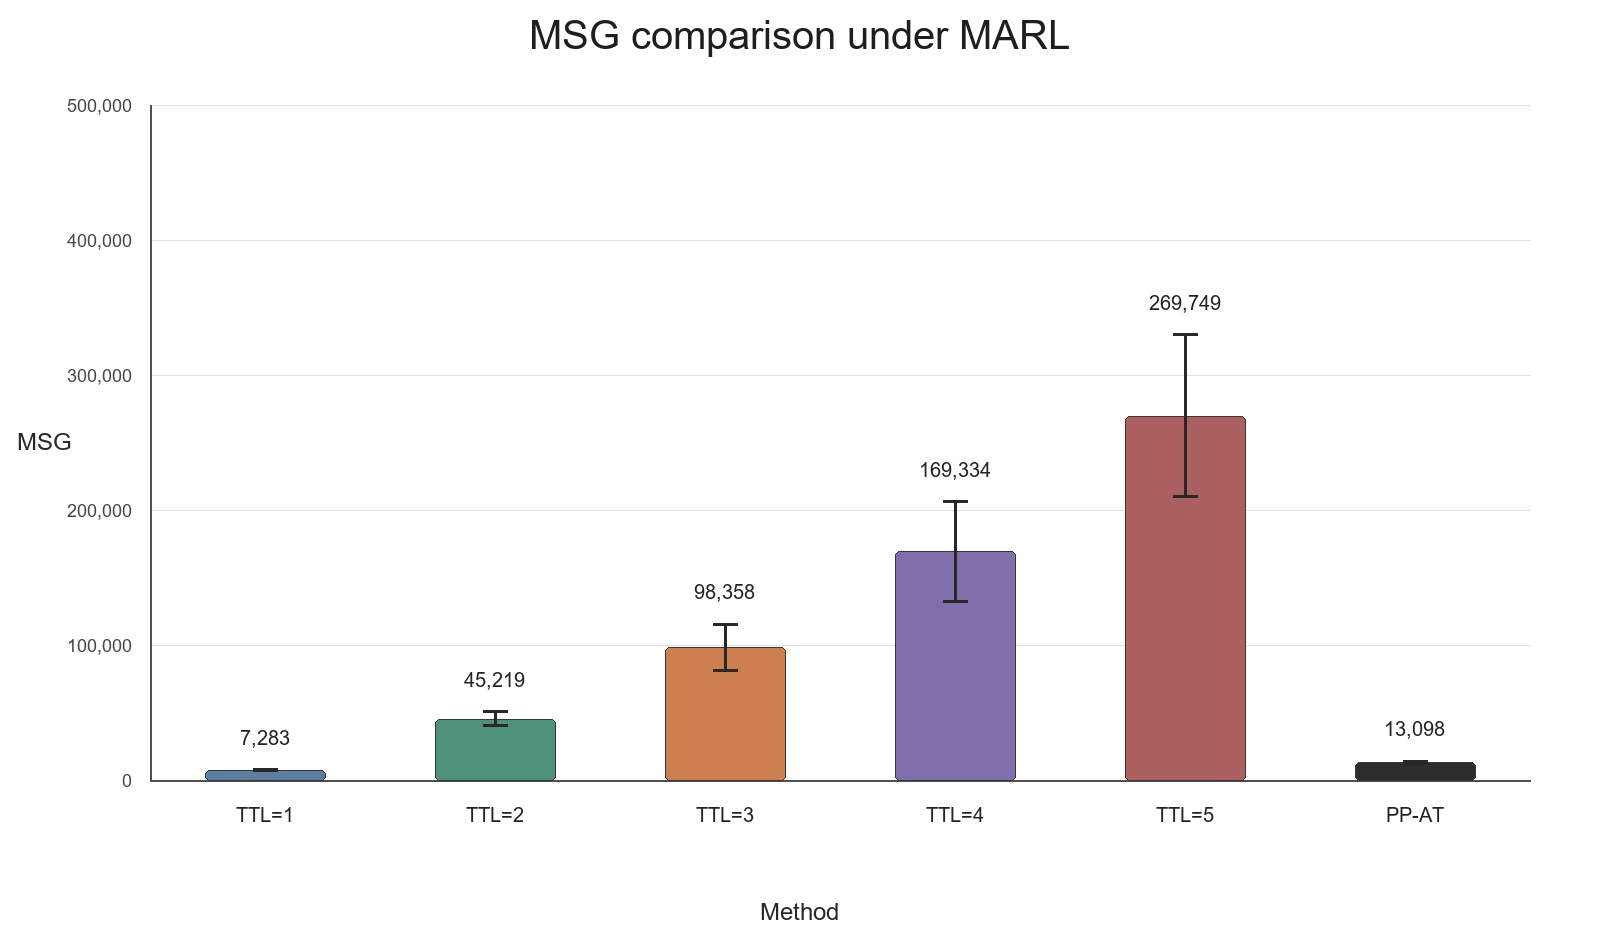
\includegraphics[width=\linewidth]{figures/marl_fig4_msg_comparison.jpg}
\captionof{figure}{MSG comparison under MARL (mean $\pm$ sample standard deviation).}
\label{fig:marl_msg_comparison}
\end{minipage}\hfill
\begin{minipage}{0.48\linewidth}
\centering
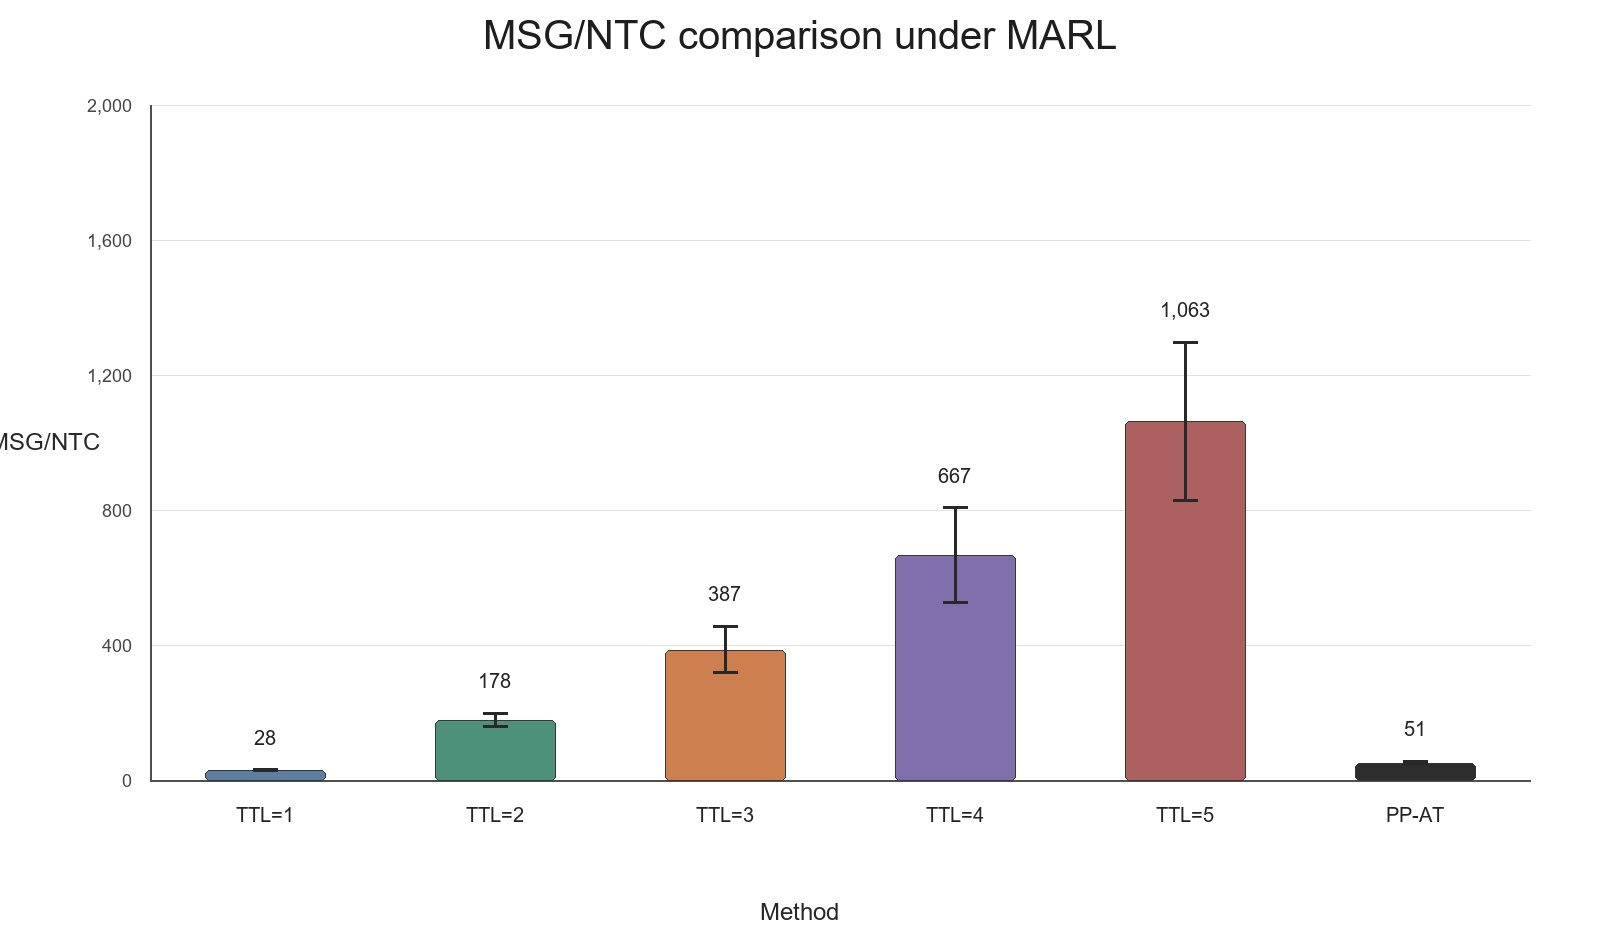
\includegraphics[width=\linewidth]{figures/marl_fig5_msg_per_ntc_comparison.jpg}
\captionof{figure}{MSG/NTC comparison under MARL (mean $\pm$ sample standard deviation).}
\label{fig:marl_msg_per_ntc_comparison}
\end{minipage}
\end{figure}



\begin{figure}[!htbp]
\centering
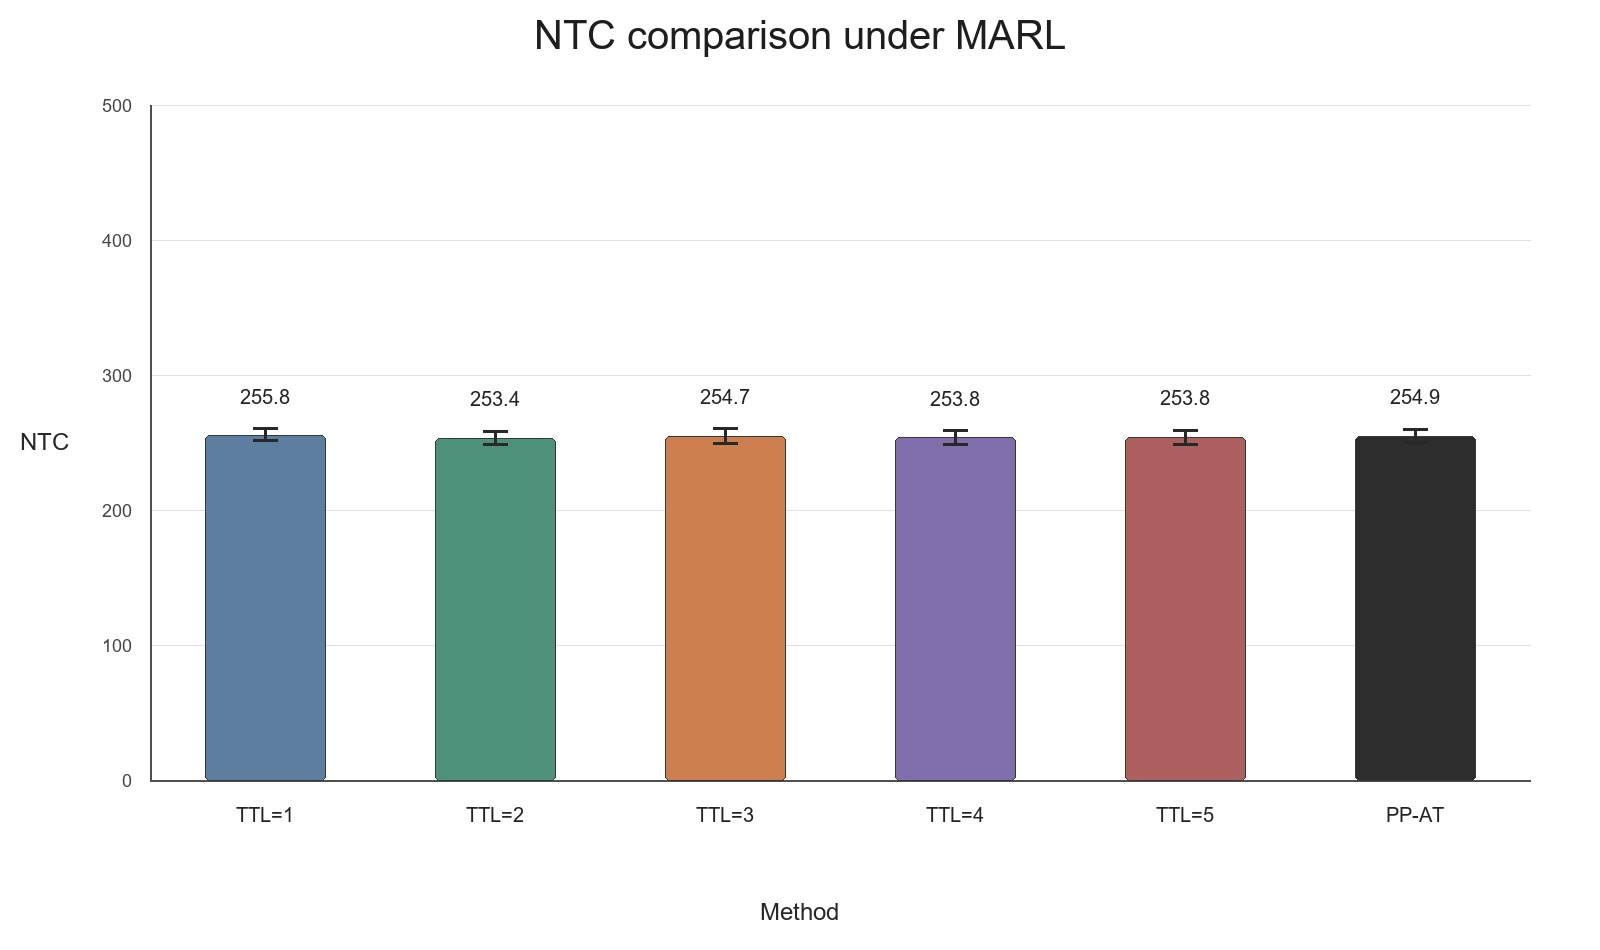
\includegraphics[width=0.62\linewidth]{figures/marl_fig6_ntc_comparison.jpg}
\caption{NTC comparison under MARL (mean $\pm$ sample standard deviation).}
\label{fig:marl_ntc_comparison}
\end{figure}


\subsection{4.3 Ablation and Robustness Analysis}
To evaluate the effects of individual components on communication overhead and task completion performance, the ablation experiments use the same task scenarios, robot settings, and 20 paired random seeds (76001--76020). All three configurations use the same MPDM allocator and message-counting rules. The service guard, an earlier rule that forces expansion when the estimated completion-time margin is small, is disabled in all configurations. State refresh and assignment awareness are each removed separately from current PP-AT. The results are presented in Table~\ref{tab:6}. Reported 95\% confidence intervals use paired Student's $t$ intervals calculated from the 20 seed-level differences (19 degrees of freedom), without adjustment for multiple comparisons. They are pointwise intervals, not simultaneous confidence guarantees. Compared with the configuration without state refresh, current PP-AT reduces MSG by 8.75\% and MSG/NTC by 8.51\%. The mean number of rejected allocation attempts decreases from 110.90 to 25.70, while mean NTC decreases by approximately 0.35\%. The paired MSG difference (PP-AT minus the ablated configuration) has a 95\% confidence interval of $[-2332.78,-834.42]$. Compared with the configuration without assignment awareness, mean MSG decreases by 4.79\%, and the mean number of rejected allocation attempts decreases from 65.40 to 25.70. However, its paired MSG confidence interval, $[-1719.47,59.17]$, includes zero, so this reduction is not statistically significant. The paired NTC confidence intervals include zero in both comparisons. These results support lower communication overhead with state refresh in this setting and fewer rejected assignments with both components, but do not establish unchanged task completion performance.

To further examine PP-AT under different environments, it is compared with Fixed TTL = 1--5 in four settings: the base environment, 100 robots, a task arrival rate of 15 tasks/s, and an initial robot resource level of 30. Each setting uses the same 20 paired random seeds across methods, with identical task scenarios and robot settings within each comparison. This seed set (79001--79020) differs from that used in the main comparison in Table~\ref{tab:main_results}. Across the four environments, PP-AT reduces mean MSG by 53.29\%--97.69\% relative to Fixed TTL = 2--5, while mean MSG/NTC also decreases. These results indicate that communication savings remain after normalization by the number of completed tasks in the tested environments. However, PP-AT has higher MSG than Fixed TTL = 1 in all four environments. Furthermore, at an arrival rate of 15 tasks/s, PP-AT reduces MSG by 88.05\% relative to Fixed TTL = 3, but mean NTC decreases by approximately 0.83\%. These trade-offs are discussed in the Discussion section. The comparison results are presented in Table~\ref{tab:fixed_robustness} and Fig.~\ref{fig:7}. Figure~\ref{fig:7} presents relative changes calculated from the method means, rather than confidence intervals. The dashed lines mark the 3\% MSG reduction and 1\% NTC decrease thresholds; negative MSG reductions indicate higher communication overhead with PP-AT.
\begin{table}[htb]
\centering
\caption{Direct Component Ablation Results Under MPDM}
\label{tab:6}
\begingroup
\small
\setlength{\tabcolsep}{4pt}
\begin{tabular}{lrrrr}
\toprule
Configuration & NTC & MSG & MSG/NTC & Rejections \\
\midrule
Current PP-AT & $253.90 \pm 4.63$ & $16510.45 \pm 1976.49$ & $64.99 \pm 7.28$ & $25.70 \pm 6.62$ \\
No state refresh & $254.80 \pm 4.58$ & $18094.05 \pm 1801.81$ & $71.03 \pm 7.21$ & $110.90 \pm 14.84$ \\
No assignment awareness & $253.35 \pm 4.04$ & $17340.60 \pm 2134.22$ & $68.41 \pm 8.03$ & $65.40 \pm 13.85$ \\
\bottomrule
\end{tabular}
\par\smallskip
\begin{minipage}{\linewidth}
\footnotesize
Values are mean $\pm$ sample standard deviation over 20 paired seeds (76001--76020), with 60 runs in total. All configurations disable the service guard. Current PP-AT enables both state refresh and assignment awareness; each ablated configuration disables only the named component. Rejections denotes rejected allocation attempts.
\end{minipage}
\endgroup
\end{table}

\begin{table}[htb]
\centering
\caption{PP-AT Relative to Fixed TTL = 2--5 Under Four Environments}
\label{tab:fixed_robustness}
\begingroup\small\setlength{\tabcolsep}{4pt}
\resizebox{\tableReferenceWidth}{!}{%
\begin{tabular}{lrrrrr}
\toprule
Environment & TTL & MSG red. (\%) & NTC change (\%) & MSG/NTC red. (\%) & Seed rate \\
\midrule
Base & 2 & 67.09 & +0.34 & 67.20 & 95\% \\
Base & 3 & 84.48 & +0.26 & 84.52 & 75\% \\
Base & 4 & 90.58 & +0.38 & 90.63 & 85\% \\
Base & 5 & 93.13 & +0.30 & 93.16 & 85\% \\
100 robots & 2 & 76.93 & +0.14 & 76.96 & 90\% \\
100 robots & 3 & 91.92 & +0.14 & 91.93 & 85\% \\
100 robots & 4 & 96.06 & +0.06 & 96.06 & 85\% \\
100 robots & 5 & 97.69 & +0.00 & 97.69 & 75\% \\
15 tasks/s & 2 & 75.21 & -0.41 & 75.09 & 65\% \\
15 tasks/s & 3 & 88.05 & -0.83 & 87.95 & 60\% \\
15 tasks/s & 4 & 92.05 & -0.47 & 92.01 & 70\% \\
15 tasks/s & 5 & 93.17 & -0.54 & 93.13 & 70\% \\
Resource 30 & 2 & 53.29 & +0.73 & 53.54 & 90\% \\
Resource 30 & 3 & 77.01 & +0.50 & 77.09 & 85\% \\
Resource 30 & 4 & 85.43 & +0.50 & 85.48 & 80\% \\
Resource 30 & 5 & 89.41 & +0.46 & 89.43 & 75\% \\
\bottomrule
\end{tabular}
}
\par\smallskip
\begin{minipage}{\linewidth}\footnotesize
Each comparison uses 20 paired seeds (79001--79020). Positive reductions indicate lower communication overhead with PP-AT; negative NTC changes indicate fewer completed tasks. Seed rate is the fraction satisfying $\mathrm{NTC}_{\mathrm{PPAT}}\geq0.99\,\mathrm{NTC}_{\mathrm{Fixed}}$. The four cases were selected before this supplement. Eighty archived PP-AT runs are paired with 400 new fixed-TTL runs. These results cover the four selected environments, not all ten environments of the earlier AT comparison.
\end{minipage}
\endgroup
\end{table}


\begin{figure}[htbp]
\centering
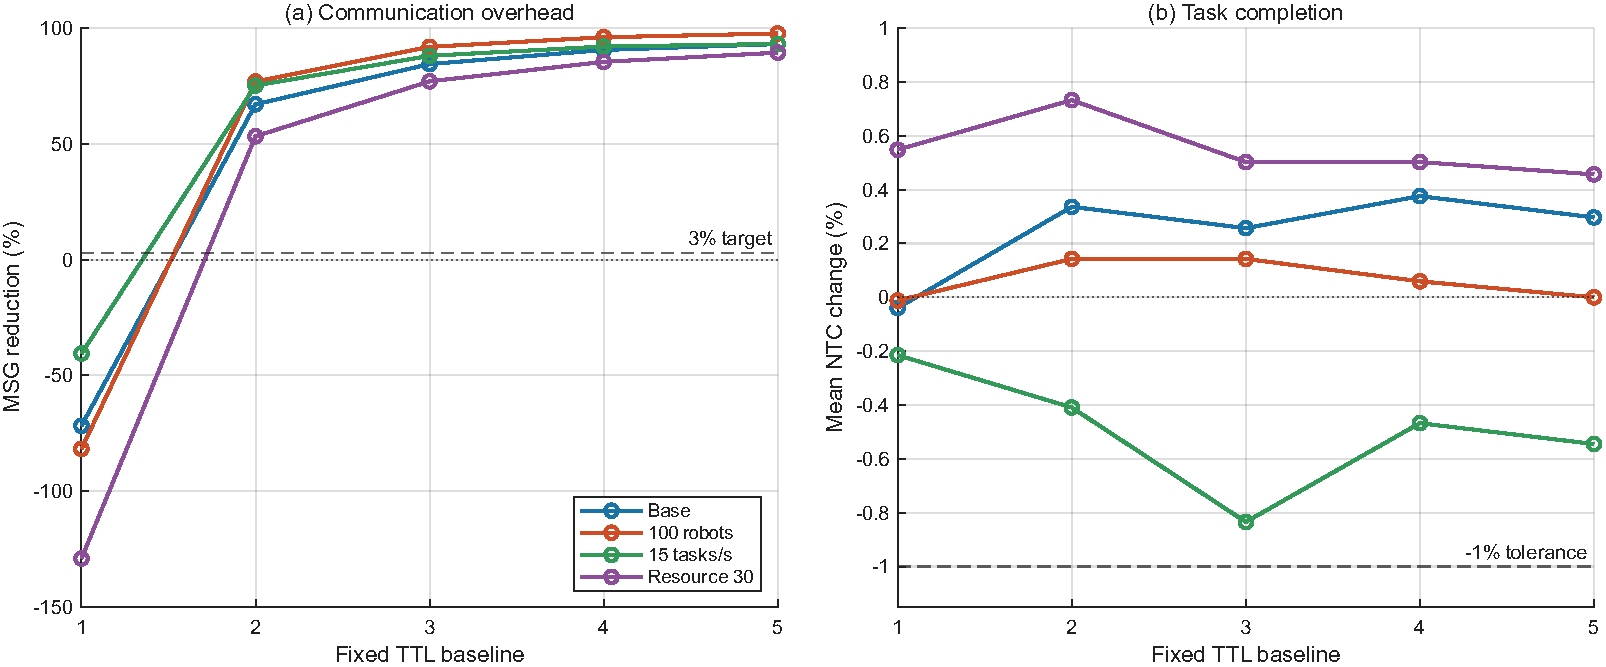
\includegraphics[width=\linewidth]{figures/fixed_robustness_comparison.pdf}
\caption{PP-AT versus fixed-TTL baselines across four MPDM environments: (a) MSG reduction; (b) NTC change.}
\label{fig:7}
\end{figure}

\FloatBarrier
\section{5. Discussion}
PP-AT reduces communication overhead relative to Fixed TTL = 2--5 in the tested environments. The decrease in MSG/NTC further indicates that these savings remain after normalization by the number of completed tasks. However, PP-AT does not outperform Fixed TTL = 1 in communication overhead. When the one-hop neighborhood already provides sufficient candidates for allocation, expansion and state maintenance can introduce additional communication without necessarily increasing task completion. Given the substantial communication savings observed relative to the larger fixed-TTL settings, the value of PP-AT lies in adapting propagation to allocation needs rather than achieving the lowest communication overhead in every environment. Moreover, the advantage of Fixed TTL = 1 in these experiments should not be interpreted as a theoretical lower bound on the overhead of all communication mechanisms.

At a task arrival rate of 15 tasks/s, PP-AT reduces MSG by 88.05\% relative to Fixed TTL = 3, but mean NTC decreases by approximately 0.83\%. Although this decrease remains below the predefined 1\% tolerance for the mean reduction, it does not imply that task completion performance is entirely unaffected. The 95\% confidence interval for the paired NTC difference excludes zero, so this decrease should not be disregarded. Propagation range, changes in candidate states, and competition among tasks may all affect allocation, but the current experiments have not isolated their individual effects. This result indicates that lower communication overhead can still be accompanied by a loss in task completion performance.

This study has several limitations. The simulation follows the localized information-sharing framework of the reference study~\cite{nayak2025limited}, but it does not exactly reproduce all of its experimental details. Furthermore, the robustness comparison against fixed TTL covers only four environments. The direct component ablations cover the base MPDM setting only; component effects under other environments and allocators remain to be examined. Future work can evaluate the method using a more complete communication model and a broader range of task conditions, and further investigate the sources of communication savings and task completion losses.



\section{6. Conclusion}
This paper proposes a protected progressive adaptive TTL mechanism, PP-AT, for multi-robot task allocation under limited information sharing. Rather than replacing existing task allocators, PP-AT serves as a communication-control mechanism. It estimates a propagation upper bound from task states and the source robot's local information, expands propagation from one hop as needed, and adjusts the propagation process through state refresh and assignment awareness. Simulations using NetFlood and MPDM show that PP-AT reduces communication overhead relative to Fixed TTL = 2--5 in the tested environments. These savings remain after normalization by the number of completed tasks. In the robustness comparisons across four environments, any decrease in mean task completion remains below 1\%. Auxiliary MARL experiments also provide preliminary evidence that the mechanism can be combined with different allocators. However, PP-AT still incurs higher communication overhead than Fixed TTL = 1, and task completion decreases in some settings. Its advantage therefore lies in the trade-off between communication overhead and task completion performance under the tested conditions, rather than a universal improvement over all fixed-TTL settings. Future work will consider more realistic communication conditions and a broader range of task scenarios to examine the method's applicability.










\subsection{Financial support and sponsorship}












\begin{thebibliography}{99}
\bibitem[Wang et al.(2024)]{wang_eepi}
Wang S, Liu Y, Qiu Y, Li S, Zhou J.
An Efficient Distributed Task Allocation Method for Maximizing Task Allocations of Multirobot Systems.
\textit{IEEE Trans. Autom. Sci. Eng.} 2024;21(3):3588--3602.
doi: \href{https://doi.org/10.1109/TASE.2023.3281577}{10.1109/TASE.2023.3281577}.

\bibitem[Nayak et al.(2025)]{nayak2025limited}
Nayak J, Mondal S, Saha S, Sarkar C.
Multi-Robot Task Allocation: Impact of Limited Information Sharing.
In: 2025 IEEE International Conference on Advanced Networks and Telecommunications Systems (ANTS). IEEE; 2025.
doi: \href{https://doi.org/10.1109/ANTS66931.2025.11429973}{10.1109/ANTS66931.2025.11429973}.

\bibitem[Yu et al.(2025)]{yu_mmoeadl}
Yu Y, Tang Q, Jiang Q, Fan Q.
A Deep Reinforcement Learning-Assisted Multimodal Multiobjective Bilevel Optimization Method for Multirobot Task Allocation.
\textit{IEEE Trans. Evol. Comput.} 2025;29(3):574--588.
doi: \href{https://doi.org/10.1109/TEVC.2025.3535954}{10.1109/TEVC.2025.3535954}.

\bibitem[Martin et al.(2026)]{martin_iterative_clustering}
Martin DR, Butler BA, Nivison S, Egerstedt M, Al Faruque MA, Khargonekar P.
Collaborative Task Allocation for Heterogeneous Multi-Robot Systems Through Iterative Clustering.
\textit{IEEE Robot. Autom. Lett.} 2026;11(1):33--40.
doi: \href{https://doi.org/10.1109/LRA.2025.3632086}{10.1109/LRA.2025.3632086}.

\bibitem[Dai et al.(2025)]{dai_heterogeneous_rl}
Dai W, Rai U, Chiun J, Cao Y, Sartoretti G.
Heterogeneous Multi-robot Task Allocation and Scheduling via Reinforcement Learning.
\textit{IEEE Robot. Autom. Lett.} 2025;10(3):2654--2661.
doi: \href{https://doi.org/10.1109/LRA.2025.3534682}{10.1109/LRA.2025.3534682}.

\bibitem[Zhang et al.(2025)]{zhang_energy_efficient}
Zhang L, Zhao J, Lamon E, Wang Y, Hong X.
Energy Efficient Multi-Robot Task Allocation Constrained by Time Window and Precedence.
\textit{IEEE Trans. Autom. Sci. Eng.} 2025;22:18162--18173.
doi: \href{https://doi.org/10.1109/TASE.2023.3312214}{10.1109/TASE.2023.3312214}.

\end{thebibliography}

\end{document}














